% Root file used ashow macros
\documentclass{beamer}
\usepackage{tikz}
\usetikzlibrary{calc}
\usetikzlibrary{decorations.pathreplacing}
\usepackage{xcolor}
\usepackage{multicol}
\usepackage{amsmath}

\setbeamertemplate{navigation symbols}{}
\setbeamersize{text margin left=0.4cm, text margin right=0.4cm}
\setlength{\multicolsep}{4pt}
% wide enough that an enumerate label in the second column of a multicols still has a
% clear word space in front of it, whatever the first column's line does
\setlength{\columnsep}{18pt}
\renewcommand{\arraystretch}{0.92}

% ================================================================
% Answer-overlay helpers
% ================================================================
\newcommand{\ablank}[1]{%
  \alt<2>{\textcolor{red}{#1}}{\underline{\phantom{#1}}}%
}
\newcommand{\ashow}[1]{\uncover<2->{\textcolor{red}{\small #1}}}
\newcommand{\ashowq}[1]{\alt<2->{\textcolor{red}{\small #1}}{?}}

% Answers drawn straight on to a TikZ diagram, revealed on overlay 2 like \ashow.
% Space is reserved on overlay 1, so the diagram does not move between slides.
\usetikzlibrary{overlay-beamer-styles}
\tikzset{
  ans/.style     = {red, thick, visible on=<2->},
  ansfill/.style = {red!15, visible on=<2->},
  anslab/.style  = {red, font=\tiny, visible on=<2->},
}

% Used by the worked solutions rather than by this deck, so that each worked
% solution is first a question with room to write in and then the answer.
\newlength{\aworkpad}
\setlength{\aworkpad}{8mm}
\newcommand{\awork}[1]{%
  \par\vspace{\aworkpad}%
  \uncover<2->{#1}%
  \par\vspace{\aworkpad}%
}

% A gap inside a TikZ node: a question mark on the first overlay and the answer in
% red on the second. Unlike \ashowq this leaves the node's own font alone, so a gap
% in a frequency tree or a Venn diagram is the same size as the numbers beside it.
\newcommand{\dgap}[1]{\alt<2->{\textcolor{red}{#1}}{?}}

% Every question list on these slides is tight, so that the diagram column and
% the question column both finish inside the slide.
\newcommand{\tightlist}{%
  \setlength{\itemsep}{0pt}\setlength{\parskip}{0pt}\setlength{\topsep}{0pt}%
}

% ================================================================
% The pictures these starters are built from.
%
% Every picture is drawn at scale 1, with its coordinates given in centimetres,
% because a TikZ scale factor shrinks the coordinates but not the text or the node
% sizes, which is what makes labels collide in a narrow column.
% ================================================================

% The outline of an open cloth bag, \bag{width}{height}, drawn from the origin.
\newcommand{\bag}[2]{%
  \draw[thick, rounded corners=3pt, fill=brown!12]
    (0,0) -- (0,#2) -- (-0.22,{#2+0.5}) -- ({#1+0.22},{#2+0.5})
       -- (#1,#2) -- (#1,0) -- cycle;}

% One counter, \ctr{x}{y}{colour}{letter}. The letter is printed on the counter so
% that the colours can still be told apart on a projector or on a photocopy.
\newcommand{\ctr}[4]{%
  \draw[fill=#3, draw=black!55, line width=0.4pt] (#1,#2) circle (0.28);
  \node[font=\tiny] at (#1,#2) {#4};}

% One chocolate in a box, \choc{x}{y}{colour}{letter}.
\newcommand{\choc}[4]{%
  \draw[fill=#3, draw=black!60, line width=0.35pt, rounded corners=1.5pt]
    ({#1-0.28},{#2-0.26}) rectangle ({#1+0.28},{#2+0.26});
  \node[font=\tiny] at (#1,#2) {#4};}

% The items on a lunch menu: \sarnie{x}{y}{letter} and \drink{x}{y}{letter}.
\newcommand{\sarnie}[3]{%
  \draw[fill=orange!25, draw=black!60, line width=0.4pt]
    ({#1-0.34},{#2-0.26}) -- ({#1+0.34},{#2-0.26}) -- (#1,{#2+0.3}) -- cycle;
  \node[font=\tiny] at (#1,{#2-0.09}) {#3};}
\newcommand{\drink}[3]{%
  \draw[fill=blue!18, draw=black!60, line width=0.4pt]
    ({#1-0.19},{#2-0.3}) -- ({#1+0.19},{#2-0.3}) -- ({#1+0.27},{#2+0.3})
    -- ({#1-0.27},{#2+0.3}) -- cycle;
  \node[font=\tiny] at (#1,#2) {#3};}

\tikzset{
  % the circles of a frequency tree, all one size so that a gap does not move them
  ftnode/.style  = {draw, circle, minimum size=0.62cm, inner sep=0pt, font=\scriptsize},
  % fill=white so that a branch label masks the branch it sits on
  ftlab/.style   = {font=\tiny, inner sep=1.5pt, fill=white},
  ftarrow/.style = {-, thick},
  % the two sets of a Venn diagram and the numbers written inside its regions
  vset/.style = {thick},
  vnum/.style = {font=\small},
  vlab/.style = {font=\scriptsize},
}

\title{Probability: Starters}
\author{}
\date{}

\begin{document}

\frame{\titlepage}

\begin{frame}[t]{Contents}
\small
\begin{columns}[T]
\column{0.5\textwidth}
\textbf{Questions and short answers}
\begin{itemize}
\item \hyperlink{q-st1}{\beamergotobutton{Starter 1}}
\item \hyperlink{q-st2}{\beamergotobutton{Starter 2}}
\item \hyperlink{q-st3}{\beamergotobutton{Starter 3}}
\item \hyperlink{q-st4}{\beamergotobutton{Starter 4}}
\item \hyperlink{q-st5}{\beamergotobutton{Starter 5}}
\item \hyperlink{q-st6}{\beamergotobutton{Starter 6}}
\item \hyperlink{q-st7}{\beamergotobutton{Starter 7}}
\item \hyperlink{q-st8}{\beamergotobutton{Starter 8}}
\item \hyperlink{q-st9}{\beamergotobutton{Starter 9}}
\end{itemize}
\column{0.5\textwidth}
\textbf{Worked solutions}
\begin{itemize}
\item \hyperlink{work-st1}{\beamergotobutton{Starter 1}}
\item \hyperlink{work-st2}{\beamergotobutton{Starter 2}}
\item \hyperlink{work-st3}{\beamergotobutton{Starter 3}}
\item \hyperlink{work-st4}{\beamergotobutton{Starter 4}}
\item \hyperlink{work-st5}{\beamergotobutton{Starter 5}}
\item \hyperlink{work-st6}{\beamergotobutton{Starter 6}}
\item \hyperlink{work-st7}{\beamergotobutton{Starter 7}}
\item \hyperlink{work-st8}{\beamergotobutton{Starter 8}}
\item \hyperlink{work-st9}{\beamergotobutton{Starter 9}}
\end{itemize}
\end{columns}
\end{frame}

%------------------------------------------------------------------
% STARTER 1: The probability scale and the words we describe it with
%------------------------------------------------------------------
\begin{frame}[t]{Starter 1}
\hypertarget{q-st1}{}
\begin{columns}[T]

\column{0.42\textwidth}
\begin{center}
\vspace{-0.8em}
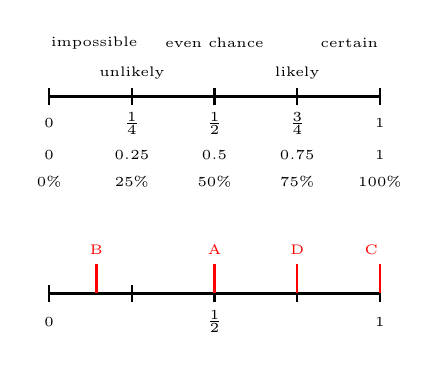
\begin{tikzpicture}[every node/.style={font=\tiny}]

% ---- The probability scale, with the words and the numbers on it ----
\draw[thick] (0,0) -- (4.2,0);
\foreach \x in {0,1.05,2.1,3.15,4.2} \draw[thick] (\x,-0.11) -- (\x,0.11);
% the words sit at two heights, so that they do not run into each other
\node[anchor=west] at (-0.10,0.68) {impossible};
\node at (2.1,0.68) {even chance};
\node[anchor=east] at (4.30,0.68) {certain};
\node at (1.05,0.30) {unlikely};
\node at (3.15,0.30) {likely};
% the same probabilities written as a fraction, a decimal and a percentage
\foreach \x/\f/\d/\p in {%
   0/$0$/$0$/$0\%$,
   1.05/$\tfrac{1}{4}$/$0.25$/$25\%$,
   2.1/$\tfrac{1}{2}$/$0.5$/$50\%$,
   3.15/$\tfrac{3}{4}$/$0.75$/$75\%$,
   4.2/$1$/$1$/$100\%$}{
  \node at (\x,-0.34) {\f};
  \node at (\x,-0.74) {\d};
  \node at (\x,-1.08) {\p};
}

% ---- An empty scale, for marking the four events on ----
\draw[thick] (0,-2.5) -- (4.2,-2.5);
\foreach \x in {0,1.05,2.1,3.15,4.2} \draw[thick] (\x,-2.61) -- (\x,-2.39);
\node at (0,-2.86) {$0$};
\node at (2.1,-2.86) {$\tfrac{1}{2}$};
\node at (4.2,-2.86) {$1$};

% the answers to question 4, marked on the empty scale
\draw[ans] (0.60,-2.50) -- (0.60,-2.12);
\node[anslab] at (0.60,-1.94) {B};
\draw[ans] (2.1,-2.50) -- (2.1,-2.12);
\node[anslab] at (2.1,-1.94) {A};
\draw[ans] (3.15,-2.50) -- (3.15,-2.12);
\node[anslab] at (3.15,-1.94) {D};
\draw[ans] (4.2,-2.50) -- (4.2,-2.12);
\node[anslab, anchor=east] at (4.30,-1.94) {C};

\end{tikzpicture}
\end{center}
\vspace{0.2em}
{\tiny\raggedright
\textbf{A} \ a fair coin lands on heads\\
\textbf{B} \ a day chosen at random is a Saturday\\
\textbf{C} \ an ordinary dice is rolled and shows a number less than $7$\\
\textbf{D} \ a counter taken from a bag of $3$ red and $1$ blue counters is red\par}

\column{0.58\textwidth}
\vspace{-1.8em}
\footnotesize
\begin{enumerate}\tightlist
\begin{multicols}{2}
  \item Write $0.25$ as a fraction in its simplest form.
        \ashow{$\tfrac{1}{4}$}
  \columnbreak
  \item Write $\dfrac{3}{5}$ as a decimal and as a percentage.
        \ashow{$0.6=60\%$}
\end{multicols}
\begin{multicols}{2}
  \item Every probability is a number from \ablank{$\;0\;$} to \ablank{$\;\;1$}.
  \columnbreak
  \item Mark events \textbf{A}, \textbf{B}, \textbf{C} and \textbf{D} on the empty scale.
\end{multicols}
  \item Complete the table.
  \begin{center}
  {\scriptsize\renewcommand{\arraystretch}{0.92}\setlength{\tabcolsep}{5pt}
  \begin{tabular}{l|c}
    Description & Probability\\ \hline
    impossible  & $0$\\
    unlikely    & between $0$ and \ablank{$0.5$}\\
    even chance & \ablank{$0.5$}\\
    likely      & between \ablank{$0.5$} and $1$\\
    certain     & \ablank{$1$}
  \end{tabular}}
  \end{center}
  \vspace{0.25em}
  \item Write a probability that is unlikely but not impossible, as a fraction, a decimal
        and a percentage.
        \ashow{Between $0$ and $0.5$, such as $\tfrac{1}{10}=0.1=10\%$.}
  \item Ravi says ``the probability that it rains tomorrow is $1.4$''. Explain why he is wrong.
        \ashow{No probability is greater than $1$; a probability of $1$ means certain.}
\end{enumerate}
\end{columns}
\end{frame}

\begin{frame}[t]{Worked Solution: Starter 1, Question 1}
\hypertarget{work-st1}{}
\textbf{Question:} Write \(0.25\) as a fraction in its simplest form.
\awork{Solution: \(0.25=\frac{25}{100}\). Divide numerator and denominator by \(25\): \(\frac{25}{100}=\frac{1}{4}\).}
\end{frame}

\begin{frame}[t]{Worked Solution: Starter 1, Question 2}
\textbf{Question:} Write \(\frac{3}{5}\) as a decimal and as a percentage.
\awork{Solution: \(\frac{3}{5}=\frac{6}{10}=0.6\). To make a percentage, multiply by \(100\): \(0.6\times100=60\%\).}
\end{frame}

\begin{frame}[t]{Worked Solution: Starter 1, Question 3}
\textbf{Question:} Every probability is a number from \underline{\hspace{1cm}} to \underline{\hspace{1cm}}.
\awork{Solution: Every probability is at least \(0\) and at most \(1\). So the gaps are \(0\) and \(1\): a probability is a number from \(0\) to \(1\).}
\end{frame}

\begin{frame}[t]{Worked Solution: Starter 1, Question 4}
\textbf{Question:} Mark events \textbf{A}, \textbf{B}, \textbf{C} and \textbf{D} on the empty scale.
\awork{Solution: \(P(A)=\frac{1}{2}=0.5\), so A is at \(0.5\). \(P(B)=\frac{1}{7}\approx0.143\), so B is near \(0\). \(P(C)=1\), so C is at \(1\). \(P(D)=\frac{3}{4}=0.75\), so D is at \(0.75\). In order from left to right: B, A, D, C.}
\end{frame}

\begin{frame}[t]{Worked Solution: Starter 1, Question 5}
\textbf{Question:} Complete the table.
\awork{Solution: The completed table is: impossible: \(0\); unlikely: between \(0\) and \(0.5\); even chance: \(0.5\); likely: between \(0.5\) and \(1\); certain: \(1\).}
\end{frame}

\begin{frame}[t]{Worked Solution: Starter 1, Question 6}
\textbf{Question:} Write a probability that is unlikely but not impossible, as a fraction, a decimal and a percentage.
\awork{Solution: Any probability strictly between \(0\) and \(0.5\) works. For example, \(\frac{1}{10}=0.1=10\%\). This is unlikely because it is less than \(0.5\), but not impossible because it is greater than \(0\).}
\end{frame}

\begin{frame}[t]{Worked Solution: Starter 1, Question 7}
\textbf{Question:} Ravi says ``the probability that it rains tomorrow is \(1.4\)''. Explain why he is wrong.
\awork{Solution: A probability cannot be greater than \(1\). \(1.4>1\), so it is not a possible probability. A probability of \(1\) would mean rain is certain; \(1.4\) would be more than certain, which is impossible.}
\end{frame}

%------------------------------------------------------------------
% STARTER 2: Probabilities from a bag of counters
%------------------------------------------------------------------
\begin{frame}[t]{Starter 2}
\hypertarget{q-st2}{}
\begin{columns}[T]

\column{0.38\textwidth}
\begin{center}
\vspace{-0.6em}
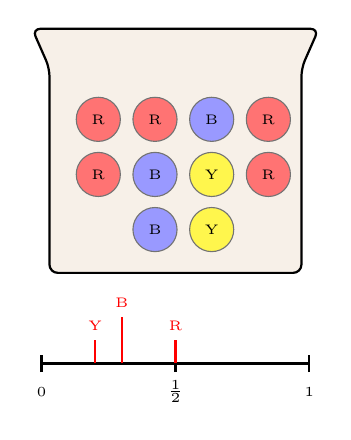
\begin{tikzpicture}[every node/.style={font=\tiny}]

% ---- A bag holding 5 red, 3 blue and 2 yellow counters ----
\bag{3.2}{2.6}
\ctr{0.62}{1.95}{red!55}{R}
\ctr{1.34}{1.95}{red!55}{R}
\ctr{2.06}{1.95}{blue!40}{B}
\ctr{2.78}{1.95}{red!55}{R}
\ctr{0.62}{1.25}{red!55}{R}
\ctr{1.34}{1.25}{blue!40}{B}
\ctr{2.06}{1.25}{yellow!70}{Y}
\ctr{2.78}{1.25}{red!55}{R}
\ctr{1.34}{0.55}{blue!40}{B}
\ctr{2.06}{0.55}{yellow!70}{Y}

% ---- A probability scale to mark the three probabilities on ----
\draw[thick] (-0.1,-1.15) -- (3.3,-1.15);
\foreach \x in {-0.1,1.6,3.3} \draw[thick] (\x,-1.26) -- (\x,-1.04);
\node at (-0.1,-1.51) {$0$};
\node at (1.6,-1.51) {$\tfrac{1}{2}$};
\node at (3.3,-1.51) {$1$};

% the answers to question 7, marked on the scale
\draw[ans] (0.58,-1.15) -- (0.58,-0.85);
\node[anslab] at (0.58,-0.67) {Y};
\draw[ans] (0.92,-1.15) -- (0.92,-0.56);
\node[anslab] at (0.92,-0.38) {B};
\draw[ans] (1.6,-1.15) -- (1.6,-0.85);
\node[anslab] at (1.6,-0.67) {R};

\end{tikzpicture}
\end{center}
\vspace{0.2em}
{\scriptsize\raggedright One counter is taken from the bag at random. The probability
that the counter is red is written $P(\text{red})$.\par}

\column{0.62\textwidth}
\vspace{-1.8em}
\footnotesize
\begin{enumerate}\tightlist
\begin{multicols}{2}
  \item Write $\dfrac{1}{2}$ as a decimal and as a percentage.
        \ashow{$0.5=50\%$}
  \columnbreak
  \item Write $30\%$ as a fraction in its simplest form.
        \ashow{$\tfrac{30}{100}=\tfrac{3}{10}$}
\end{multicols}
\begin{multicols}{2}
  \item How many counters are in the bag altogether?
        \ashow{$10$}
  \columnbreak
  \item Write $P(\text{red})$ as a fraction in its simplest form.
        \ashow{$\tfrac{5}{10}=\tfrac{1}{2}$}
\end{multicols}
\begin{multicols}{2}
  \item Write $P(\text{blue})$ as a fraction, a decimal and a percentage.
        \ashow{$\tfrac{3}{10}=0.3=30\%$}
  \columnbreak
  \item Mark $P(\text{red})$, $P(\text{blue})$ and $P(\text{yellow})$ on the
        probability scale.
\end{multicols}
\begin{multicols}{2}
  \item Write $P(\text{not red})$ as a fraction in its simplest form.
        \ashow{$\tfrac{5}{10}=\tfrac{1}{2}$}
  \columnbreak
  \item What does $P(\text{red})+P(\text{blue})+P(\text{yellow})$ come to, and why?
        \ashow{$1$; the counter is certain to be one of the three colours.}
\end{multicols}
  \item Only red counters are added to the bag, until $P(\text{red})$ is $\tfrac{3}{4}$.
        How many red counters are added?
        \ashow{$10$, giving $15$ red counters out of $20$, and $\tfrac{15}{20}=\tfrac{3}{4}$.}
\end{enumerate}
\end{columns}
\end{frame}

\begin{frame}[t]{Worked Solution: Starter 2, Question 1}
\hypertarget{work-st2}{}
\textbf{Question:} Write \(\frac{1}{2}\) as a decimal and as a percentage.
\awork{Solution: \(\frac{1}{2}=1\div2=0.5\). As a percentage: \(0.5\times100=50\%\).}
\end{frame}

\begin{frame}[t]{Worked Solution: Starter 2, Question 2}
\textbf{Question:} Write \(30\%\) as a fraction in its simplest form.
\awork{Solution: \(30\%=\frac{30}{100}\). Divide by \(10\): \(\frac{30}{100}=\frac{3}{10}\).}
\end{frame}

\begin{frame}[t]{Worked Solution: Starter 2, Question 3}
\textbf{Question:} How many counters are in the bag altogether?
\awork{Solution: Count them by colour: \(5\) red, \(3\) blue and \(2\) yellow. \(5+3+2=10\), so there are \(10\) counters altogether.}
\end{frame}

\begin{frame}[t]{Worked Solution: Starter 2, Question 4}
\textbf{Question:} Write \(P(\text{red})\) as a fraction in its simplest form.
\awork{Solution: There are \(5\) red counters out of \(10\) counters in total. \(P(\text{red})=\frac{5}{10}=\frac{1}{2}\).}
\end{frame}

\begin{frame}[t]{Worked Solution: Starter 2, Question 5}
\textbf{Question:} Write \(P(\text{blue})\) as a fraction, a decimal and a percentage.
\awork{Solution: There are \(3\) blue counters out of \(10\). \(P(\text{blue})=\frac{3}{10}=0.3=30\%\).}
\end{frame}

\begin{frame}[t]{Worked Solution: Starter 2, Question 6}
\textbf{Question:} Mark \(P(\text{red})\), \(P(\text{blue})\) and \(P(\text{yellow})\) on the probability scale.
\awork{Solution: \(P(\text{yellow})=\frac{2}{10}=0.2\), \(P(\text{blue})=\frac{3}{10}=0.3\), and \(P(\text{red})=\frac{5}{10}=0.5\). On a scale from \(0\) to \(1\), mark Y at \(0.2\), B at \(0.3\), and R at \(0.5\). So from left to right the marks are Y, B, R.}
\end{frame}

\begin{frame}[t]{Worked Solution: Starter 2, Question 7}
\textbf{Question:} Write \(P(\text{not red})\) as a fraction in its simplest form.
\awork{Solution: \(P(\text{not red})=1-P(\text{red})=1-\frac{1}{2}=\frac{1}{2}\). Alternatively, the non-red counters are \(3\) blue and \(2\) yellow, so \(\frac{5}{10}=\frac{1}{2}\).}
\end{frame}

\begin{frame}[t]{Worked Solution: Starter 2, Question 8}
\textbf{Question:} What does \(P(\text{red})+P(\text{blue})+P(\text{yellow})\) come to, and why?
\awork{Solution: \(P(\text{red})+P(\text{blue})+P(\text{yellow})=\frac{5}{10}+\frac{3}{10}+\frac{2}{10}=\frac{10}{10}=1\). This is \(1\) because every counter is red, blue or yellow, so one of these three colours is certain to be taken.}
\end{frame}

\begin{frame}[t]{Worked Solution: Starter 2, Question 9}
\textbf{Question:} Only red counters are added to the bag, until \(P(\text{red})\) is \(\frac{3}{4}\). How many red counters are added?
\awork{Solution: Let \(x\) be the number of red counters added. There were \(5\) red counters and \(10\) counters in total. After adding \(x\) red counters, red \(=5+x\) and total \(=10+x\). We need \(\frac{5+x}{10+x}=\frac{3}{4}\). Cross-multiply: \(4(5+x)=3(10+x)\), so \(20+4x=30+3x\). Thus \(x=10\). Check: \(15\) red out of \(20\) is \(\frac{15}{20}=\frac{3}{4}\). So \(10\) red counters are added.}
\end{frame}

%------------------------------------------------------------------
% STARTER 3: Comparing probabilities, and expected numbers
%------------------------------------------------------------------
\begin{frame}[t]{Starter 3}
\hypertarget{q-st3}{}
\begin{columns}[T]

\column{0.35\textwidth}
\begin{center}
\vspace{-0.6em}
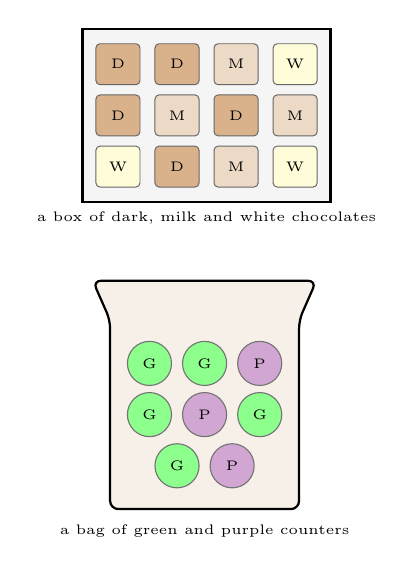
\begin{tikzpicture}[every node/.style={font=\tiny}]

% ---- A box holding 5 dark, 4 milk and 3 white chocolates ----
\draw[thick, fill=gray!8] (0,0) rectangle (3.15,2.2);
\choc{0.45}{1.75}{brown!60}{D}
\choc{1.2}{1.75}{brown!60}{D}
\choc{1.95}{1.75}{brown!30}{M}
\choc{2.7}{1.75}{yellow!15}{W}
\choc{0.45}{1.1}{brown!60}{D}
\choc{1.2}{1.1}{brown!30}{M}
\choc{1.95}{1.1}{brown!60}{D}
\choc{2.7}{1.1}{brown!30}{M}
\choc{0.45}{0.45}{yellow!15}{W}
\choc{1.2}{0.45}{brown!60}{D}
\choc{1.95}{0.45}{brown!30}{M}
\choc{2.7}{0.45}{yellow!15}{W}
\node at (1.575,-0.20) {a box of dark, milk and white chocolates};

% ---- A bag holding 5 green and 3 purple counters ----
\begin{scope}[yshift=-3.9cm, xshift=0.35cm]
\bag{2.4}{2.4}
\ctr{0.5}{1.85}{green!45}{G}
\ctr{1.2}{1.85}{green!45}{G}
\ctr{1.9}{1.85}{violet!35}{P}
\ctr{0.5}{1.2}{green!45}{G}
\ctr{1.2}{1.2}{violet!35}{P}
\ctr{1.9}{1.2}{green!45}{G}
\ctr{0.85}{0.55}{green!45}{G}
\ctr{1.55}{0.55}{violet!35}{P}
\node at (1.2,-0.28) {a bag of green and purple counters};
\end{scope}

\end{tikzpicture}
\end{center}

\column{0.65\textwidth}
\vspace{-1.8em}
\footnotesize
\begin{enumerate}\tightlist
\begin{multicols}{2}
  \item Write $\dfrac{3}{4}$ as a decimal and as a percentage.
        \ashow{$0.75=75\%$}
  \columnbreak
  \item Write $0.08$ as a percentage and as a fraction in its simplest form.
        \ashow{$8\%=\tfrac{8}{100}=\tfrac{2}{25}$}
\end{multicols}
\begin{multicols}{2}
  \item One chocolate is taken at random. Write $P(\text{white})$ in its simplest form.
        \ashow{$\tfrac{3}{12}=\tfrac{1}{4}$}
  \columnbreak
  \item Write $P(\text{not milk})$ in its simplest form.
        \ashow{$\tfrac{8}{12}=\tfrac{2}{3}$}
\end{multicols}
  \item Write $P(\text{green})$ for the bag as a fraction, a decimal and a percentage.
        \ashow{$\tfrac{5}{8}=0.625=62.5\%$}
  \item Which is more likely: a dark chocolate, or a purple counter? Show your working.
        \ashow{$\tfrac{5}{12}=\tfrac{10}{24}$ and $\tfrac{3}{8}=\tfrac{9}{24}$, so the dark chocolate.}
\begin{multicols}{2}
  \item A counter is taken from the bag at random and then replaced. This is done $200$
        times. How many green counters would you expect?
        \ashow{$\tfrac{5}{8}\times200=125$}
  \columnbreak
  \item Another bag holds only red and blue counters. It holds $12$ red counters, and
        $P(\text{red})=0.4$. How many counters are in it?
        \ashow{$12\div0.4=30$}
\end{multicols}
\end{enumerate}
\end{columns}
\end{frame}

\begin{frame}[t]{Worked Solution: Starter 3, Question 1}
\hypertarget{work-st3}{}
\textbf{Question:} Write \(\frac{3}{4}\) as a decimal and as a percentage.
\awork{Solution: \(\frac{3}{4}=3\div4=0.75\). As a percentage: \(0.75\times100=75\%\).}
\end{frame}

\begin{frame}[t]{Worked Solution: Starter 3, Question 2}
\textbf{Question:} Write \(0.08\) as a percentage and as a fraction in its simplest form.
\awork{Solution: \(0.08=8\%\). As a fraction, \(0.08=\frac{8}{100}\). Divide by \(4\): \(\frac{8}{100}=\frac{2}{25}\).}
\end{frame}

\begin{frame}[t]{Worked Solution: Starter 3, Question 3}
\textbf{Question:} One chocolate is taken at random. Write \(P(\text{white})\) in its simplest form.
\awork{Solution: There are \(3\) white chocolates. The total is \(5+4+3=12\) chocolates. \(P(\text{white})=\frac{3}{12}=\frac{1}{4}\).}
\end{frame}

\begin{frame}[t]{Worked Solution: Starter 3, Question 4}
\textbf{Question:} Write \(P(\text{not milk})\) in its simplest form.
\awork{Solution: There are \(4\) milk chocolates out of \(12\), so \(P(\text{milk})=\frac{4}{12}=\frac{1}{3}\). Therefore \(P(\text{not milk})=1-\frac{1}{3}=\frac{2}{3}\). Alternatively, the non-milk chocolates are \(5\) dark and \(3\) white, so \(\frac{8}{12}=\frac{2}{3}\).}
\end{frame}

\begin{frame}[t]{Worked Solution: Starter 3, Question 5}
\textbf{Question:} Write \(P(\text{green})\) for the bag as a fraction, a decimal and a percentage.
\awork{Solution: The bag has \(5\) green and \(3\) purple counters, so \(8\) counters in total. \(P(\text{green})=\frac{5}{8}=0.625=62.5\%\).}
\end{frame}

\begin{frame}[t]{Worked Solution: Starter 3, Question 6}
\textbf{Question:} Which is more likely: a dark chocolate, or a purple counter? Show your working.
\awork{Solution: \(P(\text{dark})=\frac{5}{12}\), because there are \(5\) dark chocolates out of \(12\). \(P(\text{purple})=\frac{3}{8}\), because there are \(3\) purple counters out of \(8\). Compare with a common denominator: \(\frac{5}{12}=\frac{10}{24}\) and \(\frac{3}{8}=\frac{9}{24}\). Since \(\frac{10}{24}>\frac{9}{24}\), a dark chocolate is more likely.}
\end{frame}

\begin{frame}[t]{Worked Solution: Starter 3, Question 7}
\textbf{Question:} A counter is taken from the bag at random and then replaced. This is done \(200\) times. How many green counters would you expect?
\awork{Solution: \(P(\text{green})=\frac{5}{8}\). Expected number \(=P(\text{green})\times200=\frac{5}{8}\times200=125\). So we would expect about \(125\) green counters.}
\end{frame}

\begin{frame}[t]{Worked Solution: Starter 3, Question 8}
\textbf{Question:} Another bag holds only red and blue counters. It holds \(12\) red counters, and \(P(\text{red})=0.4\). How many counters are in it?
\awork{Solution: Let the total number of counters be \(N\). Then \(P(\text{red})=\frac{12}{N}=0.4\). So \(12=0.4N\), and \(N=12\div0.4=30\). There are \(30\) counters in the bag.}
\end{frame}

%------------------------------------------------------------------
% STARTER 4: Listing outcomes systematically
%------------------------------------------------------------------
\begin{frame}[t]{Starter 4}
\hypertarget{q-st4}{}
\begin{columns}[T]

\column{0.32\textwidth}
\begin{center}
\vspace{-0.6em}
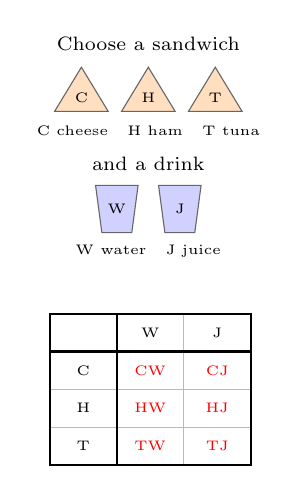
\begin{tikzpicture}[every node/.style={font=\tiny}]

% ---- The lunch deal: one sandwich and one drink ----
\node[font=\scriptsize] at (1.35,2.85) {Choose a sandwich};
\sarnie{0.5}{2.25}{C}
\sarnie{1.35}{2.25}{H}
\sarnie{2.2}{2.25}{T}
\node at (1.35,1.75) {C cheese \ \ H ham \ \ T tuna};
\node[font=\scriptsize] at (1.35,1.32) {and a drink};
\drink{0.95}{0.75}{W}
\drink{1.75}{0.75}{J}
\node at (1.35,0.22) {W water \ \ J juice};

% ---- The table every deal is listed in ----
\begin{scope}[yshift=-2.5cm, xshift=0.1cm]
\foreach \k in {0,1,2,3} \draw[gray!55] ({\k*0.85},0) -- ({\k*0.85},1.92);
\foreach \k in {0,1,2,3,4} \draw[gray!55] (0,{\k*0.48}) -- (2.55,{\k*0.48});
\draw[thick] (0,0) rectangle (2.55,1.92);
\draw[thick] (0.85,0) -- (0.85,1.92);
\draw[thick] (0,1.44) -- (2.55,1.44);
\node at (1.275,1.68) {W};
\node at (2.125,1.68) {J};
\node at (0.425,1.20) {C};
\node at (0.425,0.72) {H};
\node at (0.425,0.24) {T};
% the answers to question 4, written into the table
\node[anslab] at (1.275,1.20) {CW};
\node[anslab] at (2.125,1.20) {CJ};
\node[anslab] at (1.275,0.72) {HW};
\node[anslab] at (2.125,0.72) {HJ};
\node[anslab] at (1.275,0.24) {TW};
\node[anslab] at (2.125,0.24) {TJ};
\end{scope}

\end{tikzpicture}
\end{center}

\column{0.68\textwidth}
\vspace{-1.8em}
\footnotesize
\begin{enumerate}\tightlist
\begin{multicols}{2}
  \item Write $\dfrac{2}{5}$ as a decimal and as a percentage.
        \ashow{$0.4=40\%$}
  \columnbreak
  \item Write $65\%$ as a fraction in its simplest form.
        \ashow{$\tfrac{65}{100}=\tfrac{13}{20}$}
\end{multicols}
\begin{multicols}{2}
  \item A spinner lands on red, blue or green only. $P(\text{red})=0.35$,
        $P(\text{blue})=0.4$. Write $P(\text{green})$.
        \ashow{$1-0.35-0.4=0.25$}
  \columnbreak
  \item Complete the table to list every lunch deal.
\end{multicols}
\begin{multicols}{2}
  \item How many different lunch deals are there?
        \ashow{$6$}
  \columnbreak
  \item A deal is chosen at random. Write $P(\text{juice})$ in its simplest form.
        \ashow{$\tfrac{3}{6}=\tfrac{1}{2}$}
\end{multicols}
\begin{multicols}{2}
  \item Write $P(\text{cheese with water})$.
        \ashow{$\tfrac{1}{6}$}
  \columnbreak
  \item A third drink is added. How many deals are there now?
        \ashow{$3\times3=9$}
\end{multicols}
  \item Two fair coins are flipped. List all the outcomes systematically, then write
        $P(\text{one head and one tail})$.
        \ashow{HH, HT, TH, TT, so $\tfrac{2}{4}=\tfrac{1}{2}$}
\end{enumerate}
\end{columns}
\end{frame}

\begin{frame}[t]{Worked Solution: Starter 4, Question 1}
\hypertarget{work-st4}{}
\textbf{Question:} Write \(\frac{2}{5}\) as a decimal and as a percentage.
\awork{Solution: \(\frac{2}{5}=\frac{4}{10}=0.4\). As a percentage: \(0.4\times100=40\%\).}
\end{frame}

\begin{frame}[t]{Worked Solution: Starter 4, Question 2}
\textbf{Question:} Write \(65\%\) as a fraction in its simplest form.
\awork{Solution: \(65\%=\frac{65}{100}\). Divide numerator and denominator by \(5\): \(\frac{65}{100}=\frac{13}{20}\).}
\end{frame}

\begin{frame}[t]{Worked Solution: Starter 4, Question 3}
\textbf{Question:} A spinner lands on red, blue or green only. \(P(\text{red})=0.35\), \(P(\text{blue})=0.4\). Write \(P(\text{green})\).
\awork{Solution: The probabilities of all possible outcomes add to \(1\). \(P(\text{green})=1-0.35-0.4=0.25\).}
\end{frame}

\begin{frame}[t]{Worked Solution: Starter 4, Question 4}
\textbf{Question:} Complete the table to list every lunch deal.
\awork{Solution: There are \(3\) sandwiches: C, H, T. There are \(2\) drinks: W, J. Systematically pair each sandwich with each drink: CW, CJ, HW, HJ, TW, TJ. These are the six entries in the table.}
\end{frame}

\begin{frame}[t]{Worked Solution: Starter 4, Question 5}
\textbf{Question:} How many different lunch deals are there?
\awork{Solution: \(3\) choices of sandwich and \(2\) choices of drink, so \(3\times2=6\) different deals.}
\end{frame}

\begin{frame}[t]{Worked Solution: Starter 4, Question 6}
\textbf{Question:} A deal is chosen at random. Write \(P(\text{juice})\) in its simplest form.
\awork{Solution: Each of the \(6\) deals is equally likely. Three of them include juice: CJ, HJ, TJ. So \(P(\text{juice})=\frac{3}{6}=\frac{1}{2}\).}
\end{frame}

\begin{frame}[t]{Worked Solution: Starter 4, Question 7}
\textbf{Question:} Write \(P(\text{cheese with water})\).
\awork{Solution: There is only one deal that is cheese with water: CW. Out of \(6\) equally likely deals, \(P(\text{cheese with water})=\frac{1}{6}\).}
\end{frame}

\begin{frame}[t]{Worked Solution: Starter 4, Question 8}
\textbf{Question:} A third drink is added. How many deals are there now?
\awork{Solution: There are still \(3\) sandwiches, but now \(3\) drinks. Number of deals \(=3\times3=9\).}
\end{frame}

\begin{frame}[t]{Worked Solution: Starter 4, Question 9}
\textbf{Question:} Two fair coins are flipped. List all the outcomes systematically, then write \(P(\text{one head and one tail})\).
\awork{Solution: List the first coin then the second: HH, HT, TH, TT. There are \(4\) equally likely outcomes. The outcomes with one head and one tail are HT and TH, so there are \(2\) of them. \(P(\text{one head and one tail})=\frac{2}{4}=\frac{1}{2}\).}
\end{frame}

%------------------------------------------------------------------
% STARTER 5: A sample space of two dice
%------------------------------------------------------------------
\begin{frame}[t]{Starter 5}
\hypertarget{q-st5}{}
\begin{columns}[T]

\column{0.36\textwidth}
\vspace{-1.2em}
{\scriptsize\raggedright Two fair, ordinary dice are rolled, and the two numbers on them
are added together.\par}
\vspace{0.4em}
\begin{center}
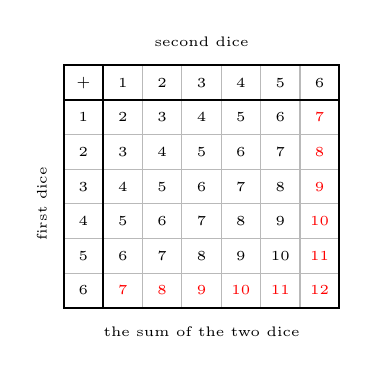
\begin{tikzpicture}[every node/.style={font=\tiny}]

% ---- The sums of two ordinary dice. The last row and the last column are the
% ---- answers to question 3, so the table is completed on the second overlay.
\foreach \k in {0,...,7} \draw[gray!55] ({\k*0.5},0) -- ({\k*0.5},3.08);
\foreach \k in {0,...,7} \draw[gray!55] (0,{\k*0.44}) -- (3.5,{\k*0.44});
\draw[thick] (0,0) rectangle (3.5,3.08);
\draw[thick] (0.5,0) -- (0.5,3.08);
\draw[thick] (0,2.64) -- (3.5,2.64);
\node at (0.25,2.86) {$+$};
\foreach \i in {1,...,6}{
  \node at (0.25,{2.86-0.44*\i}) {\i};
  \node at ({0.25+0.5*\i},2.86) {\i};
  \foreach \j in {1,...,6}{
    \pgfmathtruncatemacro{\s}{\i+\j}
    \ifnum\i<6
      \ifnum\j<6
        \node at ({0.25+0.5*\j},{2.86-0.44*\i}) {\s};
      \else
        \node[anslab] at ({0.25+0.5*\j},{2.86-0.44*\i}) {\s};
      \fi
    \else
      \node[anslab] at ({0.25+0.5*\j},{2.86-0.44*\i}) {\s};
    \fi
  }
}
\node at (1.75,-0.3) {the sum of the two dice};
\node[rotate=90, font=\tiny] at (-0.28,1.32) {first dice};
\node at (1.75,3.38) {second dice};

\end{tikzpicture}
\end{center}

\column{0.64\textwidth}
\vspace{-1.8em}
\footnotesize
\begin{enumerate}\tightlist
\begin{multicols}{2}
  \item Write $\dfrac{1}{3}$ as a decimal and as a percentage.
        \ashow{$0.\dot{3}=33.\dot{3}\%$}
  \columnbreak
  \item Write $0.36$ as a fraction in its simplest form.
        \ashow{$\tfrac{36}{100}=\tfrac{9}{25}$}
\end{multicols}
\begin{multicols}{2}
  \item Write the missing sums in the table.
  \columnbreak
  \item How many outcomes are there altogether?
        \ashow{$6\times6=36$}
\end{multicols}
\begin{multicols}{2}
  \item Write $P(\text{the sum is }7)$ in its simplest form.
        \ashow{$\tfrac{6}{36}=\tfrac{1}{6}$}
  \columnbreak
  \item Write the probability that the sum is more than $10$, in its simplest form.
        \ashow{$\tfrac{3}{36}=\tfrac{1}{12}$}
\end{multicols}
  \item Which sum is the most likely? Use its probability as a percentage to decide
        whether that sum is likely or unlikely.
        \ashow{$7$ is the most likely sum, but $\tfrac{1}{6}=16.\dot{6}\%$, which is below $50\%$, so a sum of $7$ is still unlikely.}
  \item The two dice are rolled $180$ times. How many times would you expect a sum
        of $5$?
        \ashow{$\tfrac{4}{36}=\tfrac{1}{9}$, and $\tfrac{1}{9}\times180=20$ times}
\end{enumerate}
\end{columns}
\end{frame}

\begin{frame}[t]{Worked Solution: Starter 5, Question 1}
\hypertarget{work-st5}{}
\textbf{Question:} Write \(\frac{1}{3}\) as a decimal and as a percentage.
\awork{Solution: \(\frac{1}{3}=0.333\ldots=0.\dot{3}\). As a percentage: \(0.\dot{3}\times100=33.\dot{3}\%\).}
\end{frame}

\begin{frame}[t]{Worked Solution: Starter 5, Question 2}
\textbf{Question:} Write \(0.36\) as a fraction in its simplest form.
\awork{Solution: \(0.36=\frac{36}{100}\). Divide numerator and denominator by \(4\): \(\frac{36}{100}=\frac{9}{25}\).}
\end{frame}

\begin{frame}[t]{Worked Solution: Starter 5, Question 3}
\textbf{Question:} Write the missing sums in the table.
\awork{Solution: The table shows the sum of the two dice. For the last row, the first die is \(6\), so the sums are \(6+1=7\), \(6+2=8\), \(6+3=9\), \(6+4=10\), \(6+5=11\), \(6+6=12\). For the last column, the second die is \(6\), so the remaining missing sums are \(1+6=7\), \(2+6=8\), \(3+6=9\), \(4+6=10\), \(5+6=11\). Thus the missing entries are \(7,8,9,10,11,12\) along the bottom row and \(7,8,9,10,11\) down the right column.}
\end{frame}

\begin{frame}[t]{Worked Solution: Starter 5, Question 4}
\textbf{Question:} How many outcomes are there altogether?
\awork{Solution: There are \(6\) outcomes for the first die and \(6\) for the second die. Total outcomes \(=6\times6=36\).}
\end{frame}

\begin{frame}[t]{Worked Solution: Starter 5, Question 5}
\textbf{Question:} Write \(P(\text{the sum is }7)\) in its simplest form.
\awork{Solution: The pairs giving a sum of \(7\) are \((1,6),(2,5),(3,4),(4,3),(5,2),(6,1)\), so \(6\) outcomes. \(P(\text{sum }7)=\frac{6}{36}=\frac{1}{6}\).}
\end{frame}

\begin{frame}[t]{Worked Solution: Starter 5, Question 6}
\textbf{Question:} Write the probability that the sum is more than \(10\), in its simplest form.
\awork{Solution: Sums more than \(10\) are \(11\) and \(12\). Sum \(11\): \((5,6),(6,5)\), two outcomes. Sum \(12\): \((6,6)\), one outcome. Total \(3\) outcomes. \(P(\text{sum }>10)=\frac{3}{36}=\frac{1}{12}\).}
\end{frame}

\begin{frame}[t]{Worked Solution: Starter 5, Question 7}
\textbf{Question:} Which sum is the most likely? Use its probability as a percentage to decide whether that sum is likely or unlikely.
\awork{Solution: The sum \(7\) is the most likely, because it has the most outcomes: \(6\) out of \(36\). \(P(\text{sum }7)=\frac{6}{36}=\frac{1}{6}=16.\dot{6}\%\). Since \(16.\dot{6}\%\) is less than \(50\%\), a sum of \(7\) is still unlikely, even though it is the most likely single sum.}
\end{frame}

\begin{frame}[t]{Worked Solution: Starter 5, Question 8}
\textbf{Question:} The two dice are rolled \(180\) times. How many times would you expect a sum of \(5\)?
\awork{Solution: The pairs giving a sum of \(5\) are \((1,4),(2,3),(3,2),(4,1)\), so \(4\) outcomes. \(P(\text{sum }5)=\frac{4}{36}=\frac{1}{9}\). Expected number \(=\frac{1}{9}\times180=20\). So expect \(20\) times.}
\end{frame}

%------------------------------------------------------------------
% STARTER 6: Completing a frequency tree
%------------------------------------------------------------------
\begin{frame}[t]{Starter 6}
\hypertarget{q-st6}{}
\begin{columns}[T]

\column{0.38\textwidth}
\vspace{-1.2em}
{\scriptsize\raggedright $80$ pupils sat a test. $50$ of them revised. Of the pupils who
revised, $44$ passed. Of the pupils who did not revise, $12$ passed. One of the $80$ pupils
is then chosen at random.\par}
\vspace{0.4em}
\begin{center}
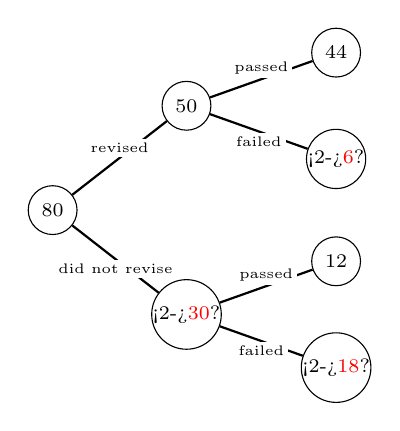
\begin{tikzpicture}

\node[ftnode] (t)  at (0,0)       {$80$};
\node[ftnode] (r)  at (1.7,1.325) {$50$};
\node[ftnode] (n)  at (1.7,-1.325){\dgap{$30$}};
\node[ftnode] (rp) at (3.6,2.0)   {$44$};
\node[ftnode] (rf) at (3.6,0.65)  {\dgap{$6$}};
\node[ftnode] (np) at (3.6,-0.65) {$12$};
\node[ftnode] (nf) at (3.6,-2.0)  {\dgap{$18$}};

\draw[ftarrow] (t) -- node[ftlab, above] {revised} (r);
\draw[ftarrow] (t) -- node[ftlab, below] {did not revise} (n);
\draw[ftarrow] (r) -- node[ftlab, above] {passed} (rp);
\draw[ftarrow] (r) -- node[ftlab, below] {failed} (rf);
\draw[ftarrow] (n) -- node[ftlab, above] {passed} (np);
\draw[ftarrow] (n) -- node[ftlab, below] {failed} (nf);

\end{tikzpicture}
\end{center}

\column{0.62\textwidth}
\vspace{-1.8em}
\footnotesize
\begin{enumerate}\tightlist
\begin{multicols}{2}
  \item Write $\dfrac{3}{8}$ as a decimal and as a percentage.
        \ashow{$0.375=37.5\%$}
  \columnbreak
  \item A bag holds $9$ red and $1$ blue counter. Is taking a red counter likely? Give
        $P(\text{red})$ as a percentage.
        \ashow{$\tfrac{9}{10}=90\%$, so likely.}
\end{multicols}
\begin{multicols}{2}
  \item Complete the frequency tree.
  \columnbreak
  \item How many pupils passed the test altogether?
        \ashow{$44+12=56$}
\end{multicols}
\begin{multicols}{2}
  \item Write $P(\text{revised})$ in its simplest form.
        \ashow{$\tfrac{50}{80}=\tfrac{5}{8}$}
  \columnbreak
  \item Write $P(\text{revised and failed})$ in its simplest form.
        \ashow{$\tfrac{6}{80}=\tfrac{3}{40}$}
\end{multicols}
  \item Write $P(\text{passed})$ as a fraction, a decimal and a percentage.
        \ashow{$\tfrac{56}{80}=\tfrac{7}{10}=0.7=70\%$}
  \item Is a pupil who revised more likely to pass than a pupil who did not revise? Use
        probabilities to explain your answer.
        \ashow{Yes: $\tfrac{44}{50}=88\%$ of those who revised passed, against $\tfrac{12}{30}=40\%$ of those who did not.}
\end{enumerate}
\end{columns}
\end{frame}

\begin{frame}[t]{Worked Solution: Starter 6, Question 1}
\hypertarget{work-st6}{}
\textbf{Question:} Write \(\frac{3}{8}\) as a decimal and as a percentage.
\awork{Solution: \(\frac{3}{8}=3\div8=0.375\). As a percentage: \(0.375\times100=37.5\%\).}
\end{frame}

\begin{frame}[t]{Worked Solution: Starter 6, Question 2}
\textbf{Question:} A bag holds \(9\) red and \(1\) blue counter. Is taking a red counter likely? Give \(P(\text{red})\) as a percentage.
\awork{Solution: There are \(9\) red counters out of \(10\) counters in total. \(P(\text{red})=\frac{9}{10}=0.9=90\%\). Since \(90\%\) is greater than \(50\%\), taking a red counter is likely.}
\end{frame}

\begin{frame}[t]{Worked Solution: Starter 6, Question 3}
\textbf{Question:} Complete the frequency tree.
\awork{Solution: The total is \(80\). \(50\) revised, so \(80-50=30\) did not revise. Of the \(50\) who revised, \(44\) passed, so \(50-44=6\) failed. Of the \(30\) who did not revise, \(12\) passed, so \(30-12=18\) failed. The missing numbers are \(30,6,18\) in the positions shown.}
\end{frame}

\begin{frame}[t]{Worked Solution: Starter 6, Question 4}
\textbf{Question:} How many pupils passed the test altogether?
\awork{Solution: Add the two passed groups: \(44\) who revised and passed plus \(12\) who did not revise and passed. \(44+12=56\). So \(56\) pupils passed.}
\end{frame}

\begin{frame}[t]{Worked Solution: Starter 6, Question 5}
\textbf{Question:} Write \(P(\text{revised})\) in its simplest form.
\awork{Solution: \(50\) pupils revised out of \(80\) pupils in total. \(P(\text{revised})=\frac{50}{80}=\frac{5}{8}\).}
\end{frame}

\begin{frame}[t]{Worked Solution: Starter 6, Question 6}
\textbf{Question:} Write \(P(\text{revised and failed})\) in its simplest form.
\awork{Solution: \(6\) pupils revised and failed. Out of \(80\) pupils, \(P(\text{revised and failed})=\frac{6}{80}=\frac{3}{40}\).}
\end{frame}

\begin{frame}[t]{Worked Solution: Starter 6, Question 7}
\textbf{Question:} Write \(P(\text{passed})\) as a fraction, a decimal and a percentage.
\awork{Solution: \(56\) pupils passed out of \(80\). \(P(\text{passed})=\frac{56}{80}=\frac{7}{10}=0.7=70\%\).}
\end{frame}

\begin{frame}[t]{Worked Solution: Starter 6, Question 8}
\textbf{Question:} Is a pupil who revised more likely to pass than a pupil who did not revise? Use probabilities to explain your answer.
\awork{Solution: Among those who revised, \(44\) out of \(50\) passed: \(\frac{44}{50}=0.88=88\%\). Among those who did not revise, \(12\) out of \(30\) passed: \(\frac{12}{30}=0.4=40\%\). Since \(88\%>40\%\), a pupil who revised was more likely to pass.}
\end{frame}

%------------------------------------------------------------------
% STARTER 7: Working backwards through a frequency tree
%------------------------------------------------------------------
\begin{frame}[t]{Starter 7}
\hypertarget{q-st7}{}
\begin{columns}[T]

\column{0.40\textwidth}
\vspace{-1.2em}
{\scriptsize\raggedright $200$ people took a driving test. $120$ of them were taking it
for the first time, and $84$ of those passed. Altogether $130$ people passed.\par}
\vspace{0.4em}
\begin{center}
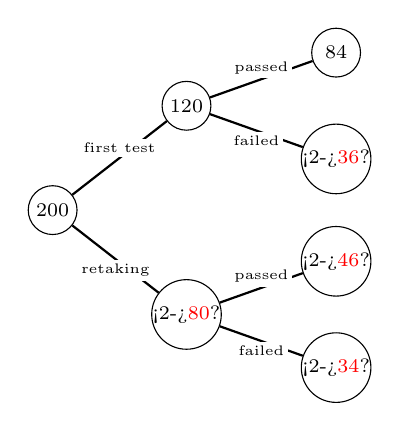
\begin{tikzpicture}

\node[ftnode] (t)  at (0,0)       {$200$};
\node[ftnode] (f)  at (1.7,1.325) {$120$};
\node[ftnode] (r)  at (1.7,-1.325){\dgap{$80$}};
\node[ftnode] (fp) at (3.6,2.0)   {$84$};
\node[ftnode] (ff) at (3.6,0.65)  {\dgap{$36$}};
\node[ftnode] (rp) at (3.6,-0.65) {\dgap{$46$}};
\node[ftnode] (rf) at (3.6,-2.0)  {\dgap{$34$}};

\draw[ftarrow] (t) -- node[ftlab, above] {first test} (f);
\draw[ftarrow] (t) -- node[ftlab, below] {retaking} (r);
\draw[ftarrow] (f) -- node[ftlab, above] {passed} (fp);
\draw[ftarrow] (f) -- node[ftlab, below] {failed} (ff);
\draw[ftarrow] (r) -- node[ftlab, above] {passed} (rp);
\draw[ftarrow] (r) -- node[ftlab, below] {failed} (rf);

\end{tikzpicture}
\end{center}

\column{0.60\textwidth}
\vspace{-1.8em}
\footnotesize
\begin{enumerate}\tightlist
\begin{multicols}{2}
  \item Write $0.65$ as a fraction in its simplest form.
        \ashow{$\tfrac{65}{100}=\tfrac{13}{20}$}
  \columnbreak
  \item Write $\dfrac{7}{8}$ as a percentage.
        \ashow{$87.5\%$}
\end{multicols}
\begin{multicols}{2}
  \item A bag holds $7$ green and $3$ red counters. Write $P(\text{green})$ as a
        percentage.
        \ashow{$\tfrac{7}{10}=70\%$}
  \columnbreak
  \item Complete the frequency tree.
\end{multicols}
\begin{multicols}{2}
  \item Write $P(\text{passed})$ in its simplest form and as a percentage.
        \ashow{$\tfrac{130}{200}=\tfrac{13}{20}=65\%$}
  \columnbreak
  \item Write the probability that a person took the test for the first time and passed.
        \ashow{$\tfrac{84}{200}=\tfrac{21}{50}$}
\end{multicols}
  \item What percentage passed on a first test, and what percentage passed on a retake?
        \ashow{$\tfrac{84}{120}=70\%$ and $\tfrac{46}{80}=57.5\%$}
  \item Jo says ``people are more likely to pass a retake, because they have had more
        practice''. Do these figures support Jo?
        \ashow{No: $70\%$ passed on a first test, but only $57.5\%$ on a retake.}
\end{enumerate}
\end{columns}
\end{frame}

\begin{frame}[t]{Worked Solution: Starter 7, Question 1}
\hypertarget{work-st7}{}
\textbf{Question:} Write \(0.65\) as a fraction in its simplest form.
\awork{Solution: \(0.65=\frac{65}{100}\). Divide numerator and denominator by \(5\): \(\frac{65}{100}=\frac{13}{20}\).}
\end{frame}

\begin{frame}[t]{Worked Solution: Starter 7, Question 2}
\textbf{Question:} Write \(\frac{7}{8}\) as a percentage.
\awork{Solution: \(\frac{7}{8}=7\div8=0.875\). As a percentage: \(0.875\times100=87.5\%\).}
\end{frame}

\begin{frame}[t]{Worked Solution: Starter 7, Question 3}
\textbf{Question:} A bag holds \(7\) green and \(3\) red counters. Write \(P(\text{green})\) as a percentage.
\awork{Solution: There are \(7\) green counters out of \(10\) counters in total. \(P(\text{green})=\frac{7}{10}=0.7=70\%\).}
\end{frame}

\begin{frame}[t]{Worked Solution: Starter 7, Question 4}
\textbf{Question:} Complete the frequency tree.
\awork{Solution: The total is \(200\). \(120\) were taking the test for the first time, so \(200-120=80\) were retaking it. Of the \(120\) first-timers, \(84\) passed, so \(120-84=36\) failed. Altogether \(130\) passed, so the number of retakers who passed is \(130-84=46\). Therefore the number of retakers who failed is \(80-46=34\). The missing numbers are \(80,36,46,34\).}
\end{frame}

\begin{frame}[t]{Worked Solution: Starter 7, Question 5}
\textbf{Question:} Write \(P(\text{passed})\) in its simplest form and as a percentage.
\awork{Solution: \(130\) people passed out of \(200\). \(P(\text{passed})=\frac{130}{200}=\frac{13}{20}=0.65=65\%\).}
\end{frame}

\begin{frame}[t]{Worked Solution: Starter 7, Question 6}
\textbf{Question:} Write the probability that a person took the test for the first time and passed.
\awork{Solution: \(84\) people took the test for the first time and passed. Out of \(200\) people, \(P(\text{first time and passed})=\frac{84}{200}=\frac{21}{50}\).}
\end{frame}

\begin{frame}[t]{Worked Solution: Starter 7, Question 7}
\textbf{Question:} What percentage passed on a first test, and what percentage passed on a retake?
\awork{Solution: First test: \(84\) passed out of \(120\), so \(\frac{84}{120}=0.7=70\%\). Retake: \(46\) passed out of \(80\), so \(\frac{46}{80}=0.575=57.5\%\).}
\end{frame}

\begin{frame}[t]{Worked Solution: Starter 7, Question 8}
\textbf{Question:} Jo says ``people are more likely to pass a retake, because they have had more practice''. Do these figures support Jo?
\awork{Solution: No. The pass rate for a first test was \(70\%\), but the pass rate for a retake was \(57.5\%\). Since \(70\%>57.5\%\), people were actually less likely to pass on a retake in these figures.}
\end{frame}

%------------------------------------------------------------------
% STARTER 8: Probabilities from a Venn diagram
%------------------------------------------------------------------
\begin{frame}[t]{Starter 8}
\hypertarget{q-st8}{}
\begin{columns}[T]

\column{0.42\textwidth}
\vspace{-1.2em}
{\scriptsize\raggedright $40$ pupils were asked which sports they play. $24$ play
football, $16$ play cricket, and $8$ play both. One pupil is then chosen at random.\par}
\vspace{0.5em}
\begin{center}
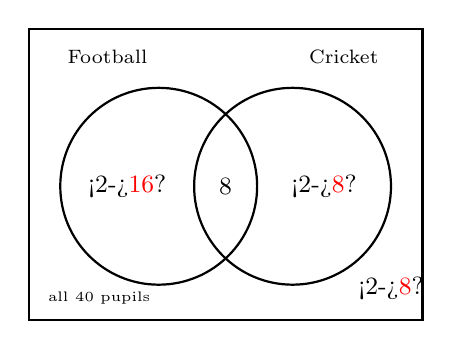
\begin{tikzpicture}[every node/.style={font=\scriptsize}]

\draw[vset] (0,0) rectangle (5.0,3.7);
\draw[vset] (1.65,1.7) circle (1.25);
\draw[vset] (3.35,1.7) circle (1.25);
\node at (1.0,3.35) {Football};
\node at (4.0,3.35) {Cricket};
\node[font=\tiny, anchor=west] at (0.12,0.28) {all $40$ pupils};

% the answers to question 3, written into the regions of the diagram
\node[vnum] at (1.25,1.7) {\dgap{$16$}};
\node[vnum] at (2.5,1.7)  {$8$};
\node[vnum] at (3.75,1.7) {\dgap{$8$}};
\node[vnum] at (4.6,0.4)  {\dgap{$8$}};

\end{tikzpicture}
\end{center}

\column{0.58\textwidth}
\vspace{-1.8em}
\footnotesize
\begin{enumerate}\tightlist
\begin{multicols}{2}
  \item Write $0.2$ as a fraction in its simplest form and as a percentage.
        \ashow{$\tfrac{1}{5}=20\%$}
  \columnbreak
  \item A caf\'e sells $4$ sandwiches and $3$ drinks. How many deals of one sandwich
        and one drink are there?
        \ashow{$4\times3=12$}
\end{multicols}
\begin{multicols}{2}
  \item How many pupils play football but not cricket?
        \ashow{$24-8=16$}
  \columnbreak
  \item Complete the Venn diagram.
\end{multicols}
\begin{multicols}{2}
  \item Write $P(\text{cricket})$ in its simplest form and as a percentage.
        \ashow{$\tfrac{16}{40}=\tfrac{2}{5}=40\%$}
  \columnbreak
  \item Write $P(\text{neither sport})$ in its simplest form.
        \ashow{$\tfrac{8}{40}=\tfrac{1}{5}$}
\end{multicols}
  \item Write $P(\text{football or cricket})$ in its simplest form and as a percentage.
        \ashow{$\tfrac{32}{40}=\tfrac{4}{5}=80\%$}
  \item $P(\text{football})+P(\text{cricket})=\tfrac{3}{5}+\tfrac{2}{5}=1$, but
        $P(\text{football or cricket})=\tfrac{4}{5}$. Explain why these are different.
        \ashow{The $8$ who play both are in both circles, so they are counted twice.}
\end{enumerate}
\end{columns}
\end{frame}

\begin{frame}[t]{Worked Solution: Starter 8, Question 1}
\hypertarget{work-st8}{}
\textbf{Question:} Write \(0.2\) as a fraction in its simplest form and as a percentage.
\awork{Solution: \(0.2=\frac{2}{10}=\frac{1}{5}\). As a percentage: \(0.2\times100=20\%\).}
\end{frame}

\begin{frame}[t]{Worked Solution: Starter 8, Question 2}
\textbf{Question:} A café sells \(4\) sandwiches and \(3\) drinks. How many deals of one sandwich and one drink are there?
\awork{Solution: For each of the \(4\) sandwiches there are \(3\) drink choices. Number of deals \(=4\times3=12\).}
\end{frame}

\begin{frame}[t]{Worked Solution: Starter 8, Question 3}
\textbf{Question:} How many pupils play football but not cricket?
\awork{Solution: \(24\) pupils play football, but \(8\) of them also play cricket. So football but not cricket \(=24-8=16\).}
\end{frame}

\begin{frame}[t]{Worked Solution: Starter 8, Question 4}
\textbf{Question:} Complete the Venn diagram.
\awork{Solution: Football only: \(24-8=16\). Both: \(8\). Cricket only: \(16-8=8\). The number who play at least one sport is \(16+8+8=32\). Since there are \(40\) pupils, neither sport is \(40-32=8\). So the regions are \(16\), \(8\), \(8\), and \(8\) outside.}
\end{frame}

\begin{frame}[t]{Worked Solution: Starter 8, Question 5}
\textbf{Question:} Write \(P(\text{cricket})\) in its simplest form and as a percentage.
\awork{Solution: \(16\) pupils play cricket out of \(40\). \(P(\text{cricket})=\frac{16}{40}=\frac{2}{5}=0.4=40\%\).}
\end{frame}

\begin{frame}[t]{Worked Solution: Starter 8, Question 6}
\textbf{Question:} Write \(P(\text{neither sport})\) in its simplest form.
\awork{Solution: \(8\) pupils play neither sport out of \(40\). \(P(\text{neither})=\frac{8}{40}=\frac{1}{5}\).}
\end{frame}

\begin{frame}[t]{Worked Solution: Starter 8, Question 7}
\textbf{Question:} Write \(P(\text{football or cricket})\) in its simplest form and as a percentage.
\awork{Solution: The number who play football or cricket is \(16+8+8=32\). So \(P(\text{football or cricket})=\frac{32}{40}=\frac{4}{5}=0.8=80\%\).}
\end{frame}

\begin{frame}[t]{Worked Solution: Starter 8, Question 8}
\textbf{Question:} \(P(\text{football})+P(\text{cricket})=\frac{3}{5}+\frac{2}{5}=1\), but \(P(\text{football or cricket})=\frac{4}{5}\). Explain why these are different.
\awork{Solution: Adding \(P(\text{football})\) and \(P(\text{cricket})\) counts the \(8\) pupils who play both sports twice. So \(\frac{3}{5}+\frac{2}{5}\) counts those pupils twice and gives \(1\). To find \(P(\text{football or cricket})\), we must count each pupil only once, so we subtract the overlap: \(\frac{3}{5}+\frac{2}{5}-\frac{8}{40}=1-\frac{1}{5}=\frac{4}{5}\).}
\end{frame}

%------------------------------------------------------------------
% STARTER 9: Sorting into a Venn diagram, then reading probabilities off it
%------------------------------------------------------------------
\begin{frame}[t]{Starter 9}
\hypertarget{q-st9}{}
\begin{columns}[T]

\column{0.42\textwidth}
\vspace{-1.2em}
{\scriptsize\raggedright One of the numbers from $1$ to $20$ is chosen at random.\par}
\vspace{0.4em}
\begin{center}
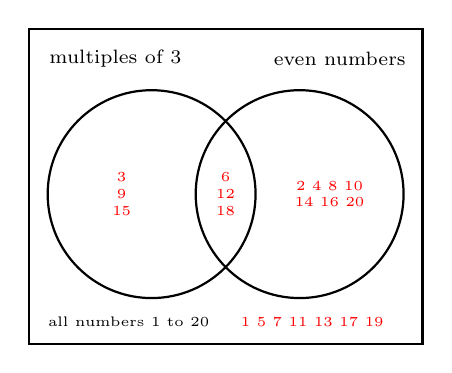
\begin{tikzpicture}[every node/.style={font=\scriptsize}]

\draw[vset] (0,0) rectangle (5.0,4.0);
\draw[vset] (1.56,1.9) circle (1.32);
\draw[vset] (3.44,1.9) circle (1.32);
\node at (1.10,3.62) {multiples of $3$};
\node at (3.95,3.62) {even numbers};
\node[font=\tiny, anchor=west] at (0.12,0.28) {all numbers $1$ to $20$};

% the answers to question 3, written into the regions of the diagram
\node[anslab, align=center] at (1.18,1.9) {$3$\\$9$\\$15$};
\node[anslab, align=center] at (2.50,1.9) {$6$\\$12$\\$18$};
\node[anslab, align=center] at (3.82,1.9) {$2$\ $4$\ $8$\ $10$\\$14$\ $16$\ $20$};
\node[anslab] at (3.60,0.28) {$1$\ $5$\ $7$\ $11$\ $13$\ $17$\ $19$};

\end{tikzpicture}
\end{center}

\column{0.58\textwidth}
\vspace{-1.8em}
\footnotesize
\begin{enumerate}\tightlist
\begin{multicols}{2}
  \item Write $\dfrac{3}{20}$ as a decimal and as a percentage.
        \ashow{$0.15=15\%$}
  \columnbreak
  \item Write $35\%$ as a fraction in its simplest form.
        \ashow{$\tfrac{35}{100}=\tfrac{7}{20}$}
\end{multicols}
\begin{multicols}{2}
  \item Write each number from $1$ to $20$ in the correct region.
  \columnbreak
  \item A number goes in the overlap when it is a multiple of \ablank{$\;6\;$}.
\end{multicols}
\begin{multicols}{2}
  \item Write $P(\text{multiple of }3)$ in its simplest form.
        \ashow{$\tfrac{6}{20}=\tfrac{3}{10}$}
  \columnbreak
  \item Write the probability that the number is neither even nor a multiple of $3$.
        \ashow{$\tfrac{7}{20}$}
\end{multicols}
  \item Is the number likely or unlikely to be a multiple of $3$? Use its probability as
        a percentage to explain.
        \ashow{$\tfrac{3}{10}=30\%$, which is below $50\%$, so unlikely.}
  \item Choose two new labels for the circles so that the overlap must be empty, and
        explain why.
        \ashow{For example ``odd'' and ``even'': no number is both odd and even.}
\end{enumerate}
\end{columns}
\end{frame}

\begin{frame}[t]{Worked Solution: Starter 9, Question 1}
\hypertarget{work-st9}{}
\textbf{Question:} Write \(\frac{3}{20}\) as a decimal and as a percentage.
\awork{Solution: \(\frac{3}{20}=\frac{15}{100}=0.15\). As a percentage: \(0.15\times100=15\%\).}
\end{frame}

\begin{frame}[t]{Worked Solution: Starter 9, Question 2}
\textbf{Question:} Write \(35\%\) as a fraction in its simplest form.
\awork{Solution: \(35\%=\frac{35}{100}\). Divide numerator and denominator by \(5\): \(\frac{35}{100}=\frac{7}{20}\).}
\end{frame}

\begin{frame}[t]{Worked Solution: Starter 9, Question 3}
\textbf{Question:} Write each number from \(1\) to \(20\) in the correct region.
\awork{Solution: Multiples of \(3\): \(3,6,9,12,15,18\). Even numbers: \(2,4,6,8,10,12,14,16,18,20\). The overlap (both even and a multiple of \(3\)) is the multiples of \(6\): \(6,12,18\). Multiples of \(3\) only: \(3,9,15\). Even only: \(2,4,8,10,14,16,20\). Neither: \(1,5,7,11,13,17,19\).}
\end{frame}

\begin{frame}[t]{Worked Solution: Starter 9, Question 4}
\textbf{Question:} A number goes in the overlap when it is a multiple of \underline{\hspace{1cm}}.
\awork{Solution: The overlap is for numbers that are both even and multiples of \(3\). Such numbers are multiples of \(6\). So the blank is \(6\).}
\end{frame}

\begin{frame}[t]{Worked Solution: Starter 9, Question 5}
\textbf{Question:} Write \(P(\text{multiple of }3)\) in its simplest form.
\awork{Solution: There are \(6\) multiples of \(3\) from \(1\) to \(20\): \(3,6,9,12,15,18\). \(P(\text{multiple of }3)=\frac{6}{20}=\frac{3}{10}\).}
\end{frame}

\begin{frame}[t]{Worked Solution: Starter 9, Question 6}
\textbf{Question:} Write the probability that the number is neither even nor a multiple of \(3\).
\awork{Solution: The numbers that are neither even nor a multiple of \(3\) are \(1,5,7,11,13,17,19\), which is \(7\) numbers. \(P(\text{neither})=\frac{7}{20}\).}
\end{frame}

\begin{frame}[t]{Worked Solution: Starter 9, Question 7}
\textbf{Question:} Is the number likely or unlikely to be a multiple of \(3\)? Use its probability as a percentage to explain.
\awork{Solution: \(P(\text{multiple of }3)=\frac{3}{10}=0.3=30\%\). Since \(30\%\) is less than \(50\%\), it is unlikely to be a multiple of \(3\).}
\end{frame}

\begin{frame}[t]{Worked Solution: Starter 9, Question 8}
\textbf{Question:} Choose two new labels for the circles so that the overlap must be empty, and explain why.
\awork{Solution: For example, label one circle ``odd numbers'' and the other ``even numbers''. No number from \(1\) to \(20\) can be both odd and even, so the overlap must be empty.}
\end{frame}

\end{document}